% Options for packages loaded elsewhere
\PassOptionsToPackage{unicode}{hyperref}
\PassOptionsToPackage{hyphens}{url}
%
\documentclass[
  ignorenonframetext,
  aspectratio=43,
]{beamer}
\usepackage{pgfpages}
\setbeamertemplate{caption}[numbered]
\setbeamertemplate{caption label separator}{: }
\setbeamercolor{caption name}{fg=normal text.fg}
\beamertemplatenavigationsymbolsempty
% Prevent slide breaks in the middle of a paragraph
\widowpenalties 1 10000
\raggedbottom
\setbeamertemplate{part page}{
  \centering
  \begin{beamercolorbox}[sep=16pt,center]{part title}
    \usebeamerfont{part title}\insertpart\par
  \end{beamercolorbox}
}
\setbeamertemplate{section page}{
  \centering
  \begin{beamercolorbox}[sep=12pt,center]{part title}
    \usebeamerfont{section title}\insertsection\par
  \end{beamercolorbox}
}
\setbeamertemplate{subsection page}{
  \centering
  \begin{beamercolorbox}[sep=8pt,center]{part title}
    \usebeamerfont{subsection title}\insertsubsection\par
  \end{beamercolorbox}
}
\AtBeginPart{
  \frame{\partpage}
}
\AtBeginSection{
  \ifbibliography
  \else
    \frame{\sectionpage}
  \fi
}
\AtBeginSubsection{
  \frame{\subsectionpage}
}
\usepackage{lmodern}
\usepackage{amssymb,amsmath}
\usepackage{ifxetex,ifluatex}
\ifnum 0\ifxetex 1\fi\ifluatex 1\fi=0 % if pdftex
  \usepackage[T1]{fontenc}
  \usepackage[utf8]{inputenc}
  \usepackage{textcomp} % provide euro and other symbols
\else % if luatex or xetex
  \usepackage{unicode-math}
  \defaultfontfeatures{Scale=MatchLowercase}
  \defaultfontfeatures[\rmfamily]{Ligatures=TeX,Scale=1}
\fi
\usetheme[]{metropolis}
\usecolortheme{seahorse}
% Use upquote if available, for straight quotes in verbatim environments
\IfFileExists{upquote.sty}{\usepackage{upquote}}{}
\IfFileExists{microtype.sty}{% use microtype if available
  \usepackage[]{microtype}
  \UseMicrotypeSet[protrusion]{basicmath} % disable protrusion for tt fonts
}{}
\makeatletter
\@ifundefined{KOMAClassName}{% if non-KOMA class
  \IfFileExists{parskip.sty}{%
    \usepackage{parskip}
  }{% else
    \setlength{\parindent}{0pt}
    \setlength{\parskip}{6pt plus 2pt minus 1pt}}
}{% if KOMA class
  \KOMAoptions{parskip=half}}
\makeatother
\usepackage{xcolor}
\IfFileExists{xurl.sty}{\usepackage{xurl}}{} % add URL line breaks if available
\IfFileExists{bookmark.sty}{\usepackage{bookmark}}{\usepackage{hyperref}}
\hypersetup{
  pdftitle={Hands-on training session 6},
  pdfauthor={Paolo Eusebi},
  hidelinks,
  pdfcreator={LaTeX via pandoc}}
\urlstyle{same} % disable monospaced font for URLs
\newif\ifbibliography
\usepackage{color}
\usepackage{fancyvrb}
\newcommand{\VerbBar}{|}
\newcommand{\VERB}{\Verb[commandchars=\\\{\}]}
\DefineVerbatimEnvironment{Highlighting}{Verbatim}{commandchars=\\\{\}}
% Add ',fontsize=\small' for more characters per line
\usepackage{framed}
\definecolor{shadecolor}{RGB}{248,248,248}
\newenvironment{Shaded}{\begin{snugshade}}{\end{snugshade}}
\newcommand{\AlertTok}[1]{\textcolor[rgb]{0.94,0.16,0.16}{#1}}
\newcommand{\AnnotationTok}[1]{\textcolor[rgb]{0.56,0.35,0.01}{\textbf{\textit{#1}}}}
\newcommand{\AttributeTok}[1]{\textcolor[rgb]{0.77,0.63,0.00}{#1}}
\newcommand{\BaseNTok}[1]{\textcolor[rgb]{0.00,0.00,0.81}{#1}}
\newcommand{\BuiltInTok}[1]{#1}
\newcommand{\CharTok}[1]{\textcolor[rgb]{0.31,0.60,0.02}{#1}}
\newcommand{\CommentTok}[1]{\textcolor[rgb]{0.56,0.35,0.01}{\textit{#1}}}
\newcommand{\CommentVarTok}[1]{\textcolor[rgb]{0.56,0.35,0.01}{\textbf{\textit{#1}}}}
\newcommand{\ConstantTok}[1]{\textcolor[rgb]{0.00,0.00,0.00}{#1}}
\newcommand{\ControlFlowTok}[1]{\textcolor[rgb]{0.13,0.29,0.53}{\textbf{#1}}}
\newcommand{\DataTypeTok}[1]{\textcolor[rgb]{0.13,0.29,0.53}{#1}}
\newcommand{\DecValTok}[1]{\textcolor[rgb]{0.00,0.00,0.81}{#1}}
\newcommand{\DocumentationTok}[1]{\textcolor[rgb]{0.56,0.35,0.01}{\textbf{\textit{#1}}}}
\newcommand{\ErrorTok}[1]{\textcolor[rgb]{0.64,0.00,0.00}{\textbf{#1}}}
\newcommand{\ExtensionTok}[1]{#1}
\newcommand{\FloatTok}[1]{\textcolor[rgb]{0.00,0.00,0.81}{#1}}
\newcommand{\FunctionTok}[1]{\textcolor[rgb]{0.00,0.00,0.00}{#1}}
\newcommand{\ImportTok}[1]{#1}
\newcommand{\InformationTok}[1]{\textcolor[rgb]{0.56,0.35,0.01}{\textbf{\textit{#1}}}}
\newcommand{\KeywordTok}[1]{\textcolor[rgb]{0.13,0.29,0.53}{\textbf{#1}}}
\newcommand{\NormalTok}[1]{#1}
\newcommand{\OperatorTok}[1]{\textcolor[rgb]{0.81,0.36,0.00}{\textbf{#1}}}
\newcommand{\OtherTok}[1]{\textcolor[rgb]{0.56,0.35,0.01}{#1}}
\newcommand{\PreprocessorTok}[1]{\textcolor[rgb]{0.56,0.35,0.01}{\textit{#1}}}
\newcommand{\RegionMarkerTok}[1]{#1}
\newcommand{\SpecialCharTok}[1]{\textcolor[rgb]{0.00,0.00,0.00}{#1}}
\newcommand{\SpecialStringTok}[1]{\textcolor[rgb]{0.31,0.60,0.02}{#1}}
\newcommand{\StringTok}[1]{\textcolor[rgb]{0.31,0.60,0.02}{#1}}
\newcommand{\VariableTok}[1]{\textcolor[rgb]{0.00,0.00,0.00}{#1}}
\newcommand{\VerbatimStringTok}[1]{\textcolor[rgb]{0.31,0.60,0.02}{#1}}
\newcommand{\WarningTok}[1]{\textcolor[rgb]{0.56,0.35,0.01}{\textbf{\textit{#1}}}}
\usepackage{graphicx,grffile}
\makeatletter
\def\maxwidth{\ifdim\Gin@nat@width>\linewidth\linewidth\else\Gin@nat@width\fi}
\def\maxheight{\ifdim\Gin@nat@height>\textheight\textheight\else\Gin@nat@height\fi}
\makeatother
% Scale images if necessary, so that they will not overflow the page
% margins by default, and it is still possible to overwrite the defaults
% using explicit options in \includegraphics[width, height, ...]{}
\setkeys{Gin}{width=\maxwidth,height=\maxheight,keepaspectratio}
% Set default figure placement to htbp
\makeatletter
\def\fps@figure{htbp}
\makeatother
\setlength{\emergencystretch}{3em} % prevent overfull lines
\providecommand{\tightlist}{%
  \setlength{\itemsep}{0pt}\setlength{\parskip}{0pt}}
\setcounter{secnumdepth}{-\maxdimen} % remove section numbering
\makeatletter
\def\verbatim@nolig@list{}
\makeatother


% fontspec requires xelatex which gives problems for me (Matt)
% \usepackage{fontspec}
% % \setmainfont[Ligatures=Historic]{TeX Gyre Pagella}
% \newfontfamily\FiraCode{Fira Code}
% \setmonofont[Contextuals={Alternate}]{Fira Code}
% \newfontfamily\Fontify[Path = ../common/]{Fontify-Regular}
% \else
% \newcommand{\Fontify}{}
% \fi



% \usepackage{fontspec}
% \setmonofont{FiraCode-Regular}[Contextuals=Alternate]
% \usepackage{listings}
% \usepackage[verbatim]{lstfiracode}
% \lstset{style=FiraCodeStyle,basicstyle=\ttfamily}
\usepackage{xspace}
\newcommand{\rlang}[0]{\texttt{R}\xspace}

\newcommand{\rpackage}[1]{\texttt{\{#1\}}}
\newcommand{\dataset}[1]{\textsl{#1}}
% \newcommand{\hotkey}[1]{#1}

% this package is conflicted with the keystroke package.
% \usepackage{statex2}

\usepackage{keystroke}
\usepackage{fvextra}
\fvset{samepage=true}
\fvset{breaklines=true}
\fvset{baselinestretch=1}
\fvset{numbers=left}
\RecustomVerbatimEnvironment{verbatim}{Verbatim}{breaklines}
\fvset{fontsize=\footnotesize}
\usepackage{ccfonts}
\makeatletter
\beamer@ignorenonframefalse
\makeatother

\usepackage{verbatim}


\title{Hands-on training session 6}
\subtitle{Meta-analyses with imperfect reference test}
\author{Paolo Eusebi}
\date{2020-02-19}

\begin{document}
\frame{\titlepage}

\hypertarget{introduction}{%
\section{Introduction}\label{introduction}}

\begin{frame}{Overview}
\protect\hypertarget{overview}{}

Date/time:

\begin{itemize}
\tightlist
\item
  20th February 2020
\item
  14.00 - 15.30
\end{itemize}

Teachers:

\begin{itemize}
\tightlist
\item
  Paolo Eusebi (presenter)
\item
  Giles Innocent
\end{itemize}

\end{frame}

\begin{frame}{Recap}
\protect\hypertarget{recap}{}

\begin{itemize}
\tightlist
\item
  Important points from previous sessions
\end{itemize}

\end{frame}

\hypertarget{session-6a-meta-analysis-of-diagnostic-test-accuracy-studies}{%
\section{Session 6a: Meta-Analysis of Diagnostic Test Accuracy
Studies}\label{session-6a-meta-analysis-of-diagnostic-test-accuracy-studies}}

\begin{frame}{DTA-MA: perfect reference test}
\protect\hypertarget{dta-ma-perfect-reference-test}{}

\begin{itemize}
\item
  There is an increasing interest in meta-analyzing data from diagnostic
  accuracy studies
\item
  The data from the primary studies are summarized in a 2-by-2
  cross-tabulation of the dichotomized test result against the true
  disease status
\end{itemize}

\begin{table}[H]
\centering\begingroup\fontsize{10}{12}\selectfont

\begin{tabular}{l|l|l}
\hline
  & D+ & D-\\
\hline
T+ & TP & FP\\
\hline
T- & FN & TN\\
\hline
\end{tabular}
\endgroup{}
\end{table}

\end{frame}

\begin{frame}{DTA-MA: perfect reference test}
\protect\hypertarget{dta-ma-perfect-reference-test-1}{}

\begin{itemize}
\tightlist
\item
  Data on magnetic resonance (MR) imaging from 10 studies on evaluation
  of lymph node metastases in patients with cervical cancer (Scheidler
  et al 1997).
\end{itemize}

\begin{table}[H]
\centering\begingroup\fontsize{10}{12}\selectfont

\begin{tabular}{l|r|r|r|r}
\hline
StudyID & TP & FP & FN & TN\\
\hline
Study 1 & 9 & 2 & 2 & 44\\
\hline
Study 2 & 3 & 6 & 5 & 32\\
\hline
Study 3 & 3 & 2 & 1 & 16\\
\hline
Study 4 & 3 & 1 & 12 & 44\\
\hline
Study 5 & 1 & 1 & 6 & 16\\
\hline
Study 6 & 7 & 2 & 22 & 167\\
\hline
Study 7 & 12 & 4 & 4 & 29\\
\hline
Study 8 & 23 & 5 & 14 & 230\\
\hline
Study 9 & 8 & 5 & 5 & 53\\
\hline
Study 10 & 16 & 2 & 2 & 22\\
\hline
\end{tabular}
\endgroup{}
\end{table}

\end{frame}

\begin{frame}{DTA-MA: perfect reference test}
\protect\hypertarget{dta-ma-perfect-reference-test-2}{}

\begin{itemize}
\tightlist
\item
  Forest plot of sensitivity
\end{itemize}

\includegraphics{Adv6_MetaAnalysis_files/figure-beamer/unnamed-chunk-3-1.pdf}

\end{frame}

\begin{frame}{DTA-MA: perfect reference test}
\protect\hypertarget{dta-ma-perfect-reference-test-3}{}

\begin{itemize}
\tightlist
\item
  Forest plot of specificity
\end{itemize}

\includegraphics{Adv6_MetaAnalysis_files/figure-beamer/unnamed-chunk-4-1.pdf}

\end{frame}

\begin{frame}{DTA-MA: perfect reference test}
\protect\hypertarget{dta-ma-perfect-reference-test-4}{}

\begin{itemize}
\tightlist
\item
  Data points with confidence ellipses on a ROC space
\end{itemize}

\includegraphics{Adv6_MetaAnalysis_files/figure-beamer/unnamed-chunk-5-1.pdf}

\end{frame}

\begin{frame}{DTA Meta-analysis}
\protect\hypertarget{dta-meta-analysis}{}

Two main framework:

\begin{itemize}
\item
  Hierarchical Summary ROC (Rutter and Gatsonis 2001)
\item
  Bivariate analysis of sensitivity and specificity (Reitsma et
  al.~2005)
\end{itemize}

\end{frame}

\begin{frame}[fragile]{DTA-MA: bivariate analysis of sensitivity and
specificity}
\protect\hypertarget{dta-ma-bivariate-analysis-of-sensitivity-and-specificity}{}

\begin{Shaded}
\begin{Highlighting}[]
\NormalTok{fit.reitsma <-}\StringTok{ }\KeywordTok{reitsma}\NormalTok{(MRI2)}
\KeywordTok{print}\NormalTok{(}\KeywordTok{summary}\NormalTok{(fit.reitsma)[}\DecValTok{1}\NormalTok{], }\DataTypeTok{digits =} \DecValTok{2}\NormalTok{)}
\end{Highlighting}
\end{Shaded}

\begin{verbatim}
## $coefficients
##                   Estimate Std. Error     z Pr(>|z|)
## tsens.(Intercept)    0.230       0.39  0.59     0.55
## tfpr.(Intercept)    -2.801       0.32 -8.64     0.00
## sensitivity          0.557         NA    NA       NA
## false pos. rate      0.057         NA    NA       NA
##                   95%ci.lb 95%ci.ub
## tsens.(Intercept)   -0.534     0.99
## tfpr.(Intercept)    -3.437    -2.17
## sensitivity          0.370     0.73
## false pos. rate      0.031     0.10
\end{verbatim}

\end{frame}

\begin{frame}{DTA-MA: bivariate analysis of sensitivity and specificity}
\protect\hypertarget{dta-ma-bivariate-analysis-of-sensitivity-and-specificity-1}{}

\includegraphics{Adv6_MetaAnalysis_files/figure-beamer/unnamed-chunk-7-1.pdf}

\end{frame}

\begin{frame}[fragile]{DTA-MA: bivariate analysis of sensitivity and
specificity}
\protect\hypertarget{dta-ma-bivariate-analysis-of-sensitivity-and-specificity-2}{}

The function returns also HSROC parameters

\begin{Shaded}
\begin{Highlighting}[]
\KeywordTok{print}\NormalTok{(}\KeywordTok{summary}\NormalTok{(fit.reitsma)[}\DecValTok{20}\NormalTok{], }\DataTypeTok{digits =} \DecValTok{2}\NormalTok{)}
\end{Highlighting}
\end{Shaded}

\begin{verbatim}
## $coef_hsroc
## $coef_hsroc$Theta
## [1] -1.5
## 
## $coef_hsroc$Lambda
## [1] 3.4
## 
## $coef_hsroc$beta
## [1] -0.26
## 
## $coef_hsroc$sigma2theta
## [1] 0.62
## 
## $coef_hsroc$sigma2alpha
## [1] 0.72
\end{verbatim}

\end{frame}

\begin{frame}{DTA-MA: bivariate analysis of sensitivity and specificity}
\protect\hypertarget{dta-ma-bivariate-analysis-of-sensitivity-and-specificity-3}{}

This is because Bivariate and HSROC approaches are equivalent when
covariates are not included (Harbord et al.~2007)

\begin{itemize}
\item
  Parameter estimates from either model can be used to produce a summary
  operating point, an SROC curve, confidence regions, or prediction
  regions.
\item
  The choice between these parameterizations depends partly on the
  degrees of and reasons for between-study heterogeneity and the
  treshold effect.
\end{itemize}

\end{frame}

\begin{frame}{DTA-MA: bivariate analysis of sensitivity and specificity}
\protect\hypertarget{dta-ma-bivariate-analysis-of-sensitivity-and-specificity-4}{}

\begin{figure}
\centering
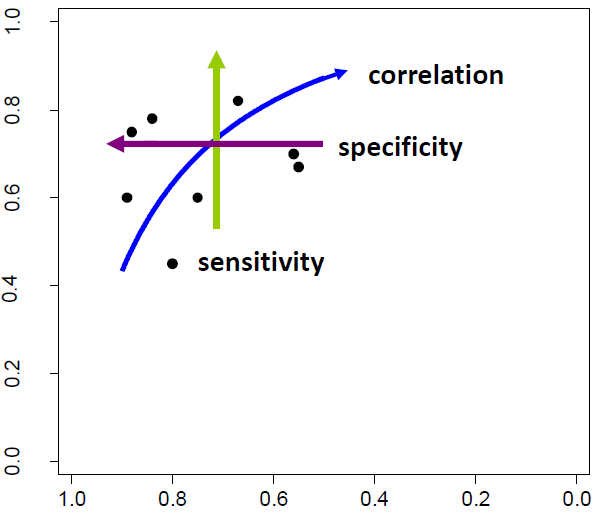
\includegraphics{/Users/paoloeusebi/Desktop/Lavoro/Harmony/Athens2020/DTA Meta-analysis/images/bivariate.png}
\caption{Alt text}
\end{figure}

\end{frame}

\begin{frame}{DTA-MA: hierarchical summary ROC (HSROC)}
\protect\hypertarget{dta-ma-hierarchical-summary-roc-hsroc}{}

\begin{figure}
\centering
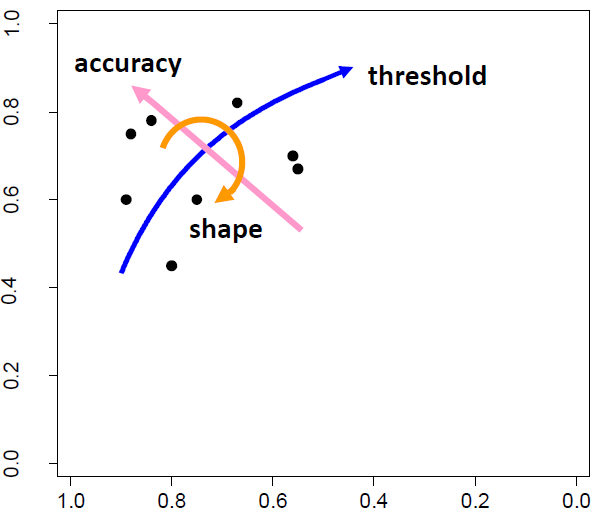
\includegraphics{/Users/paoloeusebi/Desktop/Lavoro/Harmony/Athens2020/DTA Meta-analysis/images/hsroc.png}
\caption{Alt text}
\end{figure}

\end{frame}

\begin{frame}[fragile]{DTA-MA: hierarchical summary ROC (HSROC)}
\protect\hypertarget{dta-ma-hierarchical-summary-roc-hsroc-1}{}

Use of HSROC package

\begin{Shaded}
\begin{Highlighting}[]
\KeywordTok{HSROC}\NormalTok{(}\DataTypeTok{data =}\NormalTok{ MRI,}
      \DataTypeTok{iter.num =} \DecValTok{5000}\NormalTok{,}
      \DataTypeTok{init =}\NormalTok{ init)}

\KeywordTok{HSROCSummary}\NormalTok{(}\DataTypeTok{data =}\NormalTok{ MRI,}
             \DataTypeTok{burn_in =} \DecValTok{1000}\NormalTok{,}
             \DataTypeTok{Thin =} \DecValTok{2}\NormalTok{,}
             \DataTypeTok{print_plot =}\NormalTok{ T)}
\end{Highlighting}
\end{Shaded}

\end{frame}

\begin{frame}[fragile]{DTA-MA: hierarchical summary ROC (HSROC)}
\protect\hypertarget{dta-ma-hierarchical-summary-roc-hsroc-2}{}

\begin{itemize}
\tightlist
\item
  The HSROC package allows to run multiple chains
\end{itemize}

\begin{Shaded}
\begin{Highlighting}[]
\KeywordTok{HSROCSummary}\NormalTok{(}\DataTypeTok{data =}\NormalTok{ MRI,}
             \DataTypeTok{burn_in =} \DecValTok{1000}\NormalTok{,}
             \DataTypeTok{Thin =} \DecValTok{2}\NormalTok{,}
             \DataTypeTok{print_plot =}\NormalTok{ T, }
             \DataTypeTok{chain =} \KeywordTok{list}\NormalTok{(dir.chain1, dir.chain2, dir.chain3))}
\end{Highlighting}
\end{Shaded}

A single call to the function HSROCSummary will summarize all chains (3
in our example).

\end{frame}

\begin{frame}{Exercise}
\protect\hypertarget{exercise}{}

Fit a HSROC model assuming imperfect reference for the data on Tibsit

Use rjags and HSROC

\end{frame}

\end{document}
